\section{Design}


\subsection{Overordnet System Design}
\noindent Dette afsnit repræsenterer hvordan modulerne ønskes at kommunikere med hinanden samt give et overblik over hvor meget der kommunikeres mellem modulerne i de forskellige stadier. Der vil i dette afsnit indgå 4 User stories til at repræsentere systemets design. Disse User Stories er relevante for design, da de involverer alle moduler samtidigt og giver et indblik i kommunikationen på tværs af systemet.

\noindent Herunder ses et sekvensdiagram for User Story 7-10 - Load. Her ses hvordan det ønskes at de forskellige moduler kommunikerer på tværs af systemet når bruger loade et save fra databasen.
\begin{figure}[h]
\centering
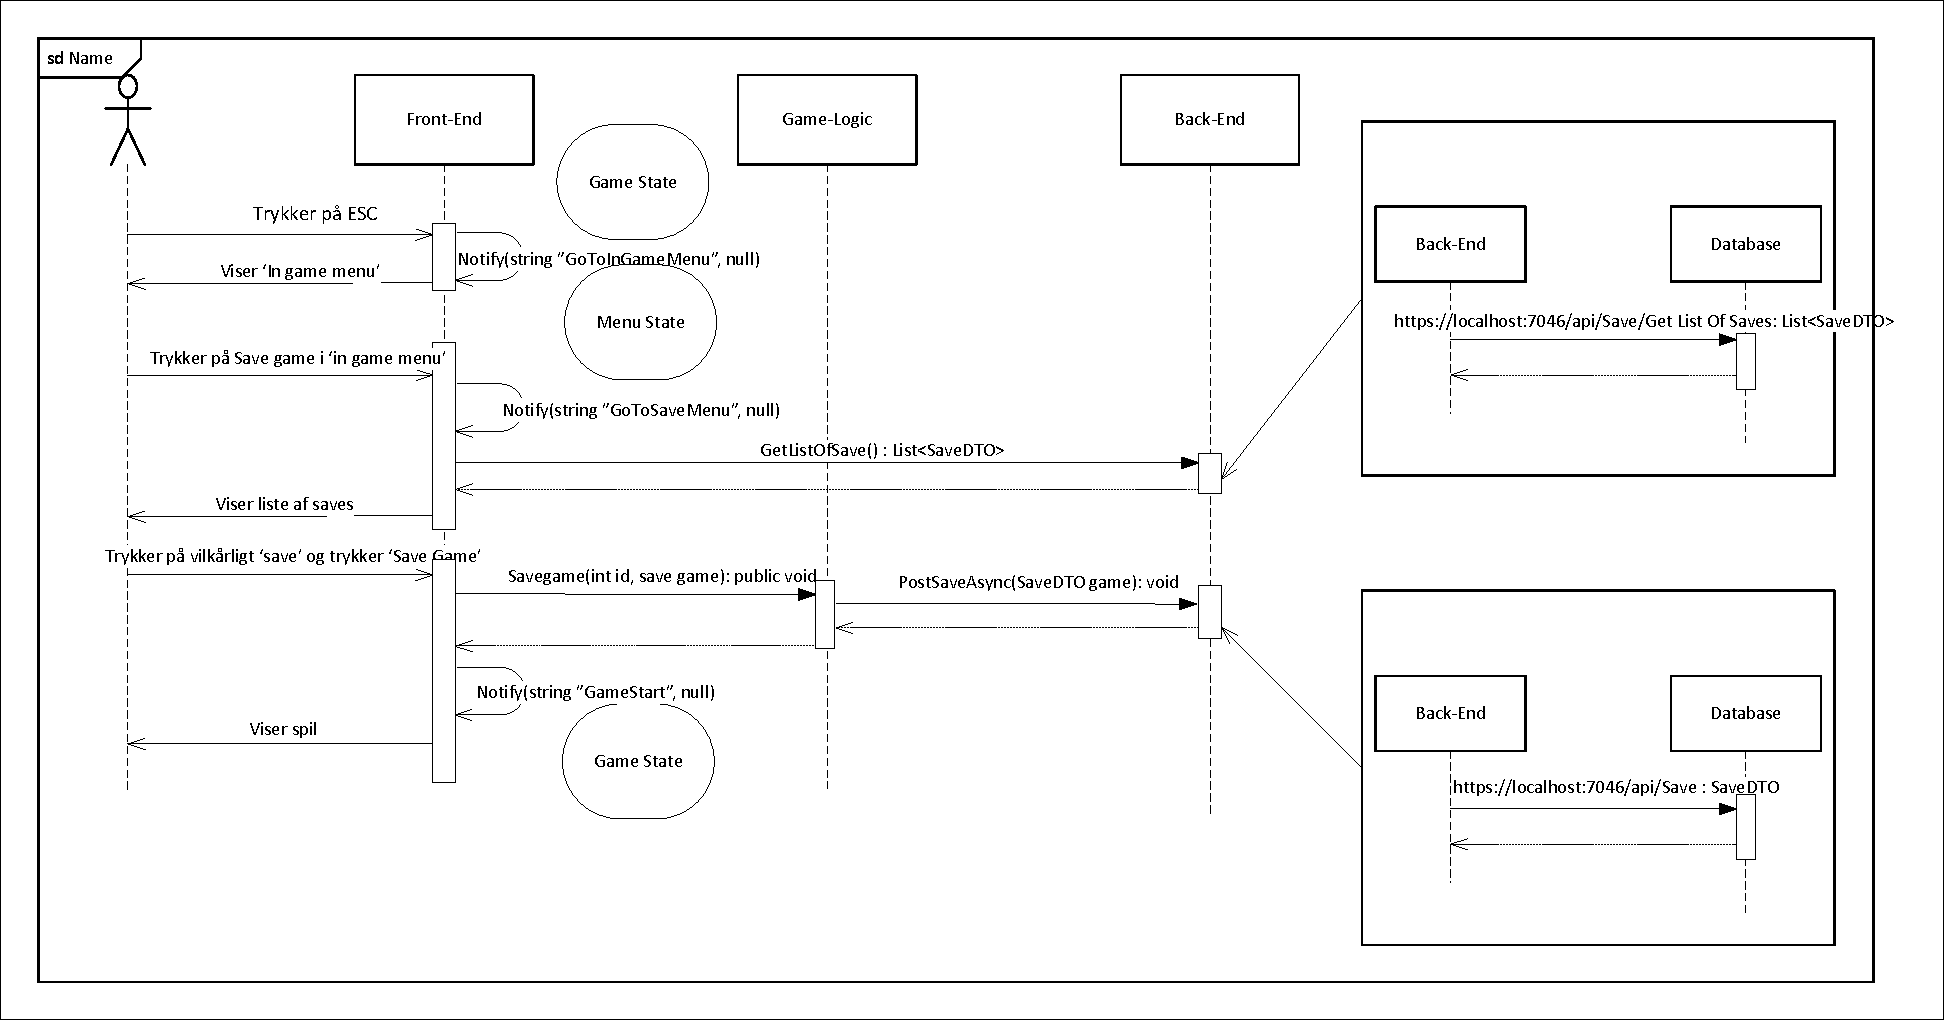
\includegraphics[width = \textwidth]{02-Body/Images/Arkitektur - SD Save Game}
\caption{SD diagram for User Story 7-10. Diagrammet viser hvordan det ønskes at systemet overordnet skal kommunikere på tværs af hindanden når bruger skal gemme sit aktuelle save}
\label{fig:Arkitektur-SD-SaveGame}
\end{figure}

\noindent Herunder ses et sekvensdiagram for User Story 17-18 - Load. Her ses hvordan det ønskes at de forskellige moduler kommunikerer på tværs af systemet når bruger gemme et save i databasen.
\begin{figure}[h]
\centering
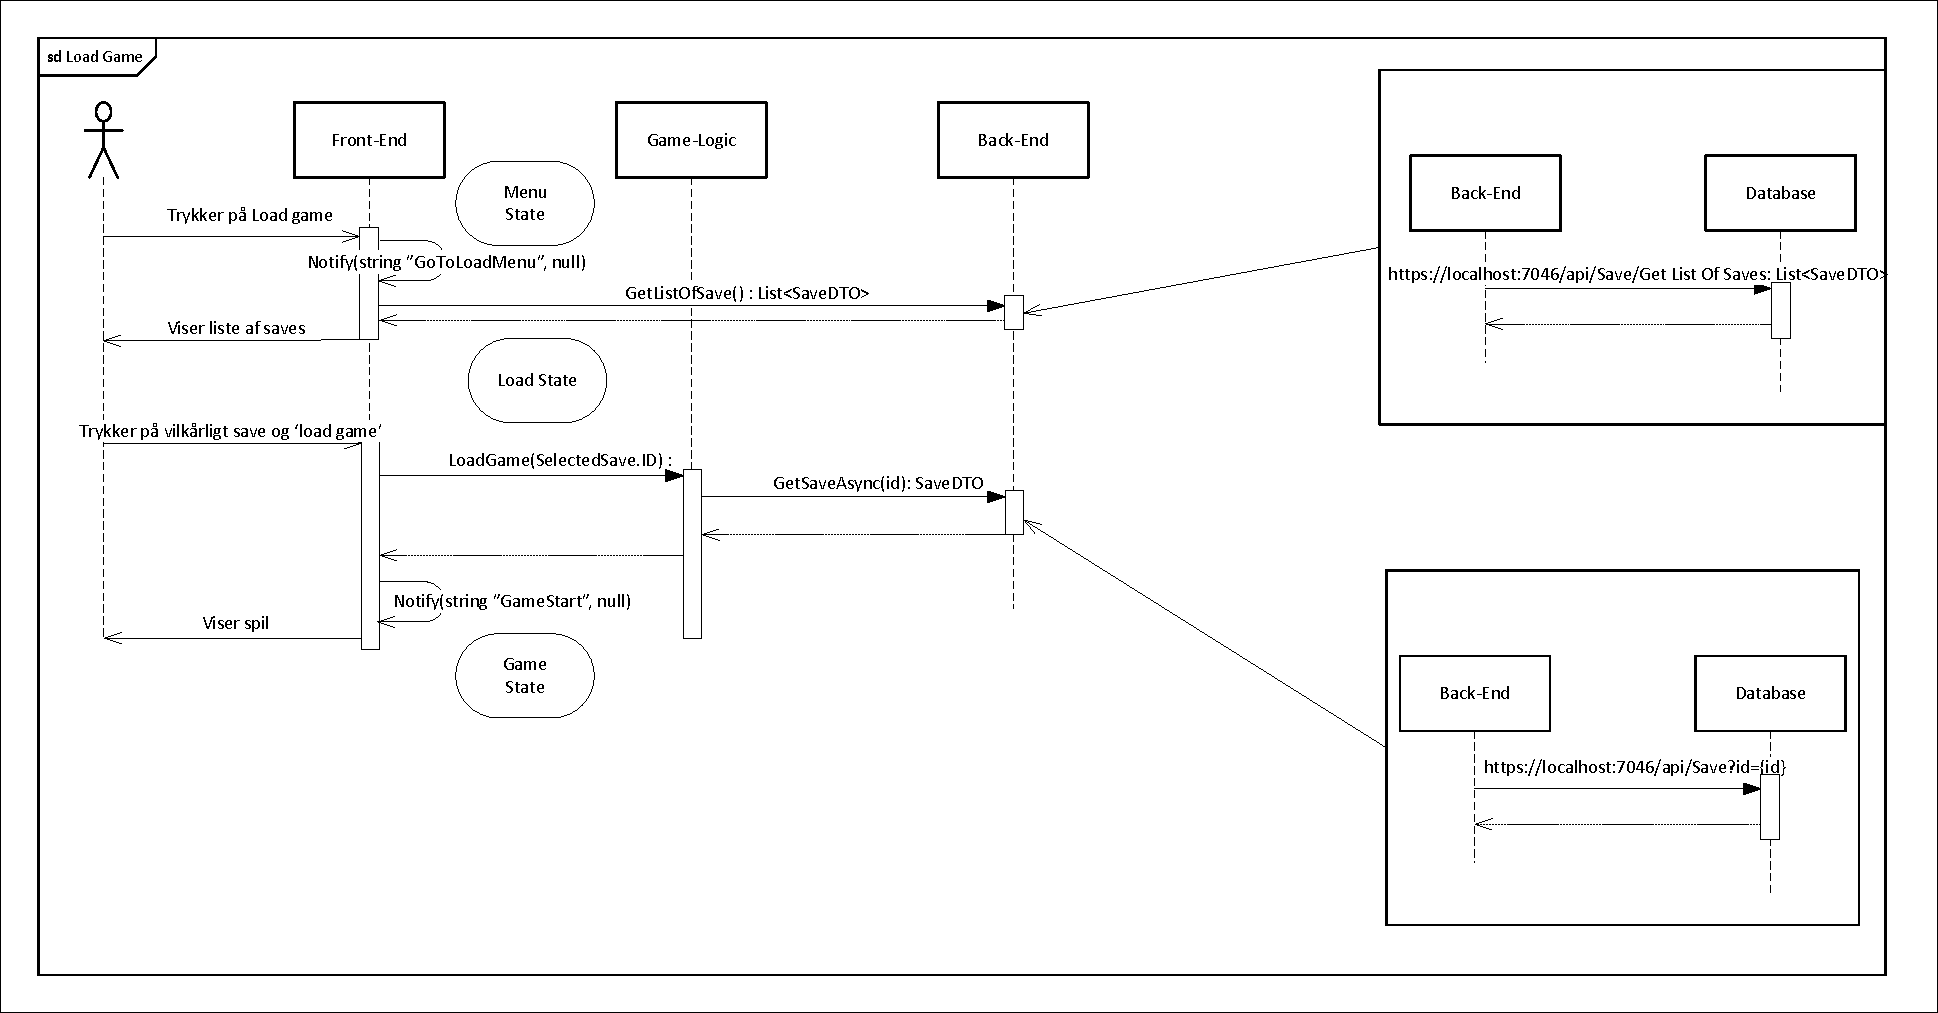
\includegraphics[width = \textwidth]{02-Body/Images/Arkitektur - SD Load Game}
\caption{SD diagram for User Story 17-18. Diagrammet viser hvordan systemet overordnet skal kommunikere på tværs når bruger skal loade sit aktuelle save. }
\label{fig:Arkitektur-SD-LoadGame}
\end{figure}

\noindent Herunder ses et sekvensdiagram for User Story 1 - Log in. Her ses hvordan det ønskes at de forskellige moduler kommunikerer på tværs af systemet når bruger skal logge ind.
\begin{figure}[h]
\centering
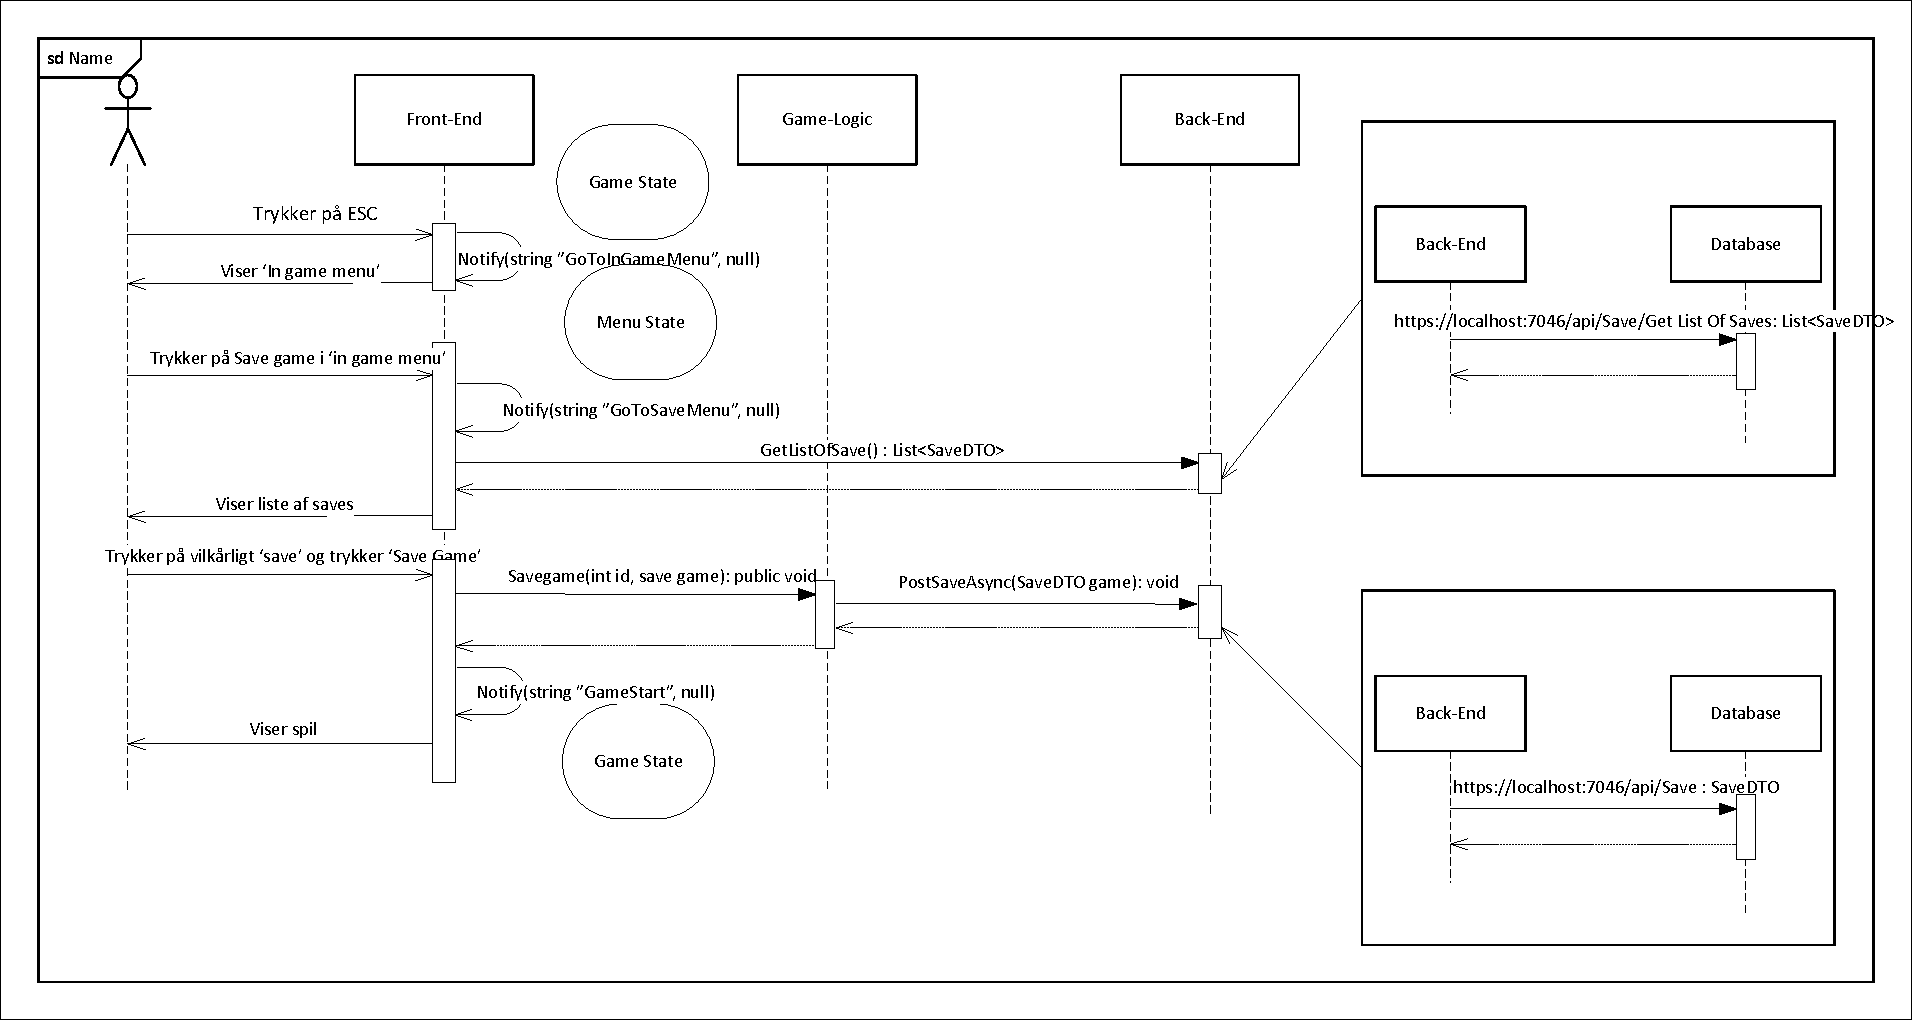
\includegraphics[width = \textwidth]{02-Body/Images/Arkitektur - SD Login}
\caption{SD diagram for User Story 1. Diagrammet viser hvordan systemet overordnet skal kommunikere på tværs når bruger skal logge ind}
\label{fig:Arkitektur-SD-Login}
\end{figure}

\noindent  Herunder ses et sekvensdiagram for User Story 2 - Opret Bruger. Her ses hvordan det ønskes at de forskellige moduler kommunikerer på tværs af systemet når bruger skal oprette en bruger i systemet.
\begin{figure}[h]
\centering
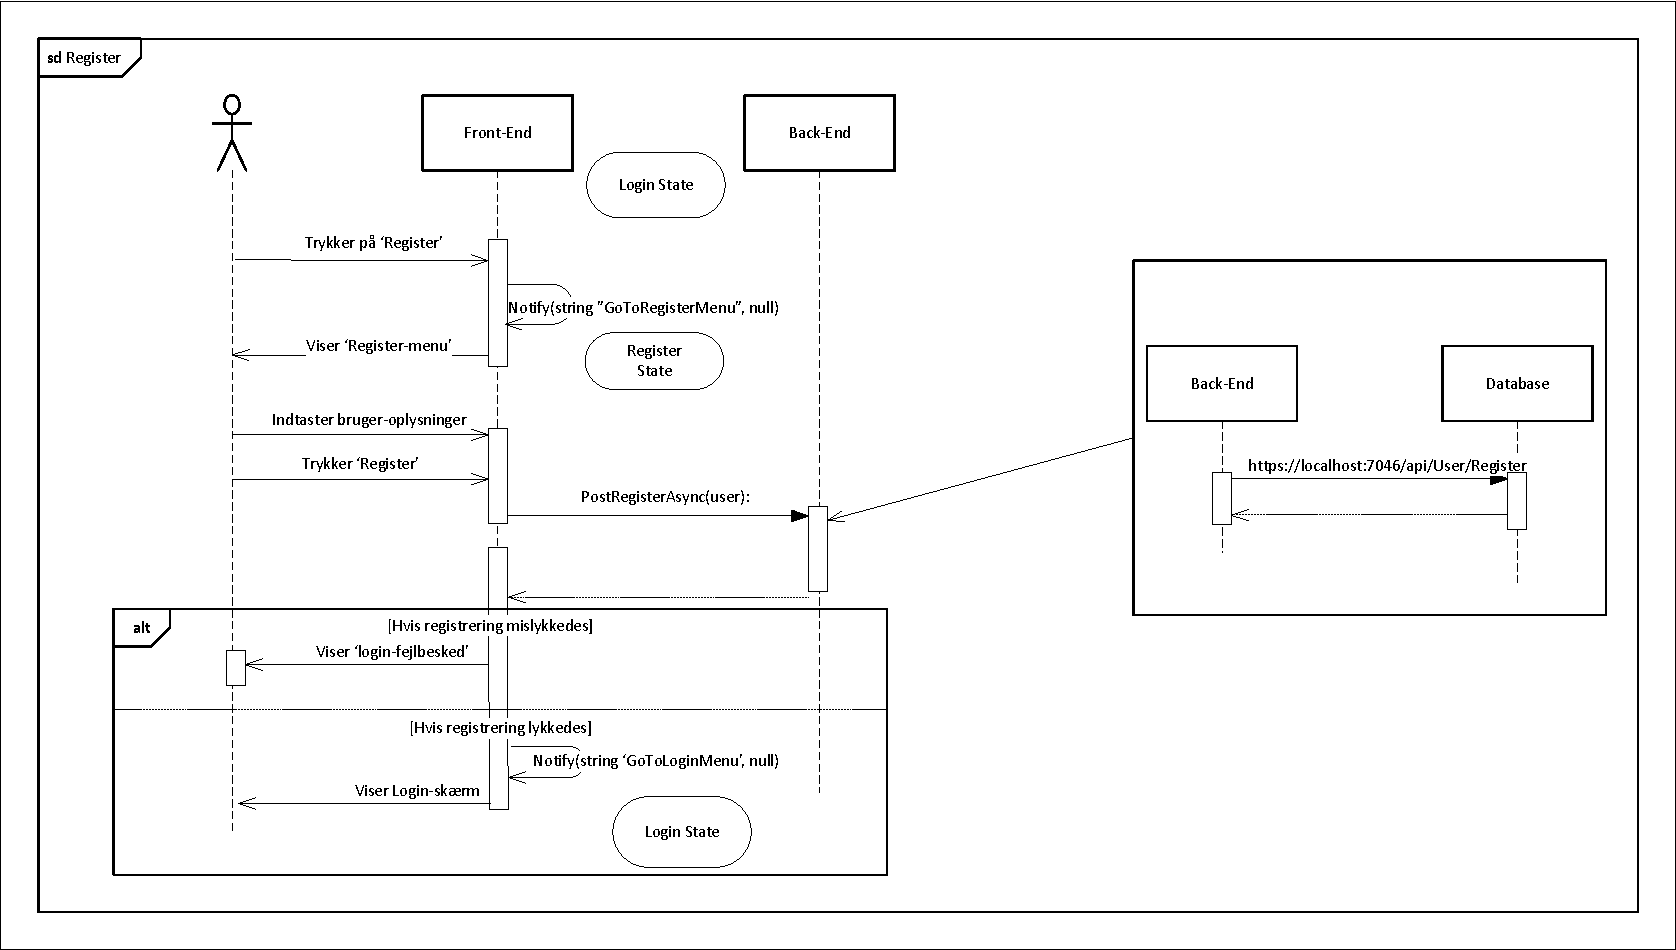
\includegraphics[width = \textwidth]{02-Body/Images/Arkitektur - SD Register}
\caption{SD diagram for User Story 2. Diagrammet viser hvordan systemet overordnet skal kommunikere på tværs når bruger skal oprette en bruger i systemet}
\label{fig:Arkitektur-SD-Register}
\end{figure}

